\documentclass[border=0pt]{standalone}
% newcommands.tex

\newcommand{\enq}{\texttt{enq}}
\newcommand{\deq}{\texttt{deq}}
\newcommand{\pput}{\texttt{PUT}}
\newcommand{\get}{\texttt{GET}}
\newcommand{\vs}{\texttt{vis}}
\newcommand{\so}{\texttt{so}}
\newcommand{\arb}{\texttt{ar}}
\newcommand{\rf}{\texttt{rf}}

% example
\newcommand{\po}[2]{\draw [->, thick] (#1) to node[above] {\Large{\so}} (#2);}
\newcommand{\pva}[2]{\draw [->, thick] (#1) to node[above] {$\Large{\so},\Large{\vs},\Large{\arb}$} (#2);}
\newcommand{\pbva}[2]{\draw [->, thick] (#1) to node[above] {$\Large{\so}$} node[below] {$\Large{\vs},\Large{\arb}$} (#2);}
\newcommand{\pv}[2]{\draw [->, thick] (#1) to node[above] {\Large{\so}} node[below] {\Large{\vs}} (#2);}
\newcommand{\evis}[2]{\draw [->, thick] (#1) to node[above, sloped, near end] {\Large{\vs}} (#2);}
\newcommand{\mvis}[2]{\draw [->, thick] (#1) to node[above, sloped] {\Large{\vs}} (#2);}
\newcommand{\ar}[2]{\draw [->, thick, allow upside down] (#1) to node[above, sloped] {\Large{\arb}} (#2);}
\newcommand{\va}[2]{\draw [->, thick, allow upside down] (#1) to node[above, sloped] {$\Large{\vs},\Large{\arb}$} (#2);}
\newcommand{\vab}[2]{\draw [->, thick, allow upside down] (#1) to node[below, sloped, near end] {$\Large{\vs},\Large{\arb}$} (#2);}
\newcommand{\vae}[2]{\draw [->, thick, allow upside down] (#1) to node[above, sloped, near end] {$\Large{\vs},\Large{\arb}$} (#2);}
\newcommand{\vas}[2]{\draw [->, thick, allow upside down] (#1) to node[sloped, near start, above] {$\Large{\vs},\Large{\arb}$} (#2);}

% serialization
\newcommand{\scc}[2]{\draw [->, very thick] (#1) to (#2);}
\newcommand{\rva}[2]{\draw [->, thick, allow upside down] (#1) to node[above, sloped] {$\Large{\rf},\Large{\vs},\Large{\arb}$} (#2);}
\newcommand{\rvb}[2]{\draw [->, thick, allow upside down] (#1) to node[below, sloped] {$\Large{\rf},\Large{\vs},\Large{\arb}$} (#2);}

\pagestyle{empty} % Remove page numbering
\usepackage[left=68pt, right=0pt, top=72pt, bottom=0pt]{geometry}

\begin{document}
	\pgfplotsset{height=140pt, width=200pt}
	% https://tex.stackexchange.com/questions/6388/how-to-scale-a-tikzpicture-to-textwidth
	\makeatletter
	\newsavebox{\measure@tikzpicture}
	\NewEnviron{scaletikzpicturetowidth}[1]{%
		\def\tikz@width{#1}%
		\def\tikzscale{1}\begin{lrbox}{\measure@tikzpicture}%
			\BODY
		\end{lrbox}%
		\pgfmathparse{#1/\wd\measure@tikzpicture}%
		\edef\tikzscale{\pgfmathresult}%
		\BODY
	}
	\makeatother
	
	\begin{minipage}{0.48\textwidth}
		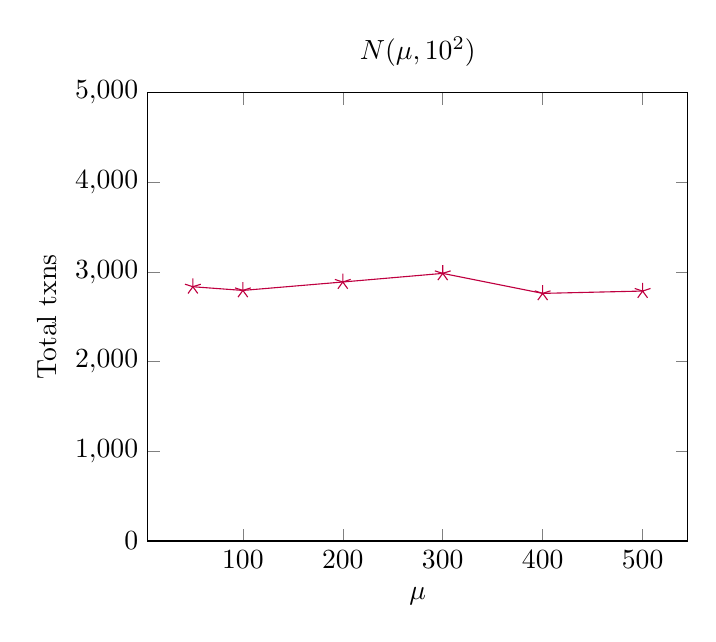
\begin{tikzpicture}
			\begin{axis}[
				title={$N(\mu,10^2)$},
				x tick label style={draw=none},
				xlabel={$\mu$},
				ylabel={Total txns},
				ymin=0,
				ymax=5000,
				]
				\addplot[color=purple,mark=star,mark size=3pt] coordinates {(50,2836) (100,2795) (200,2889) (300,2985) (400,2762) (500,2788)};
			\end{axis}
		\end{tikzpicture}
	\end{minipage}
	\hspace{-60pt}
	\begin{minipage}{0.48\textwidth}
		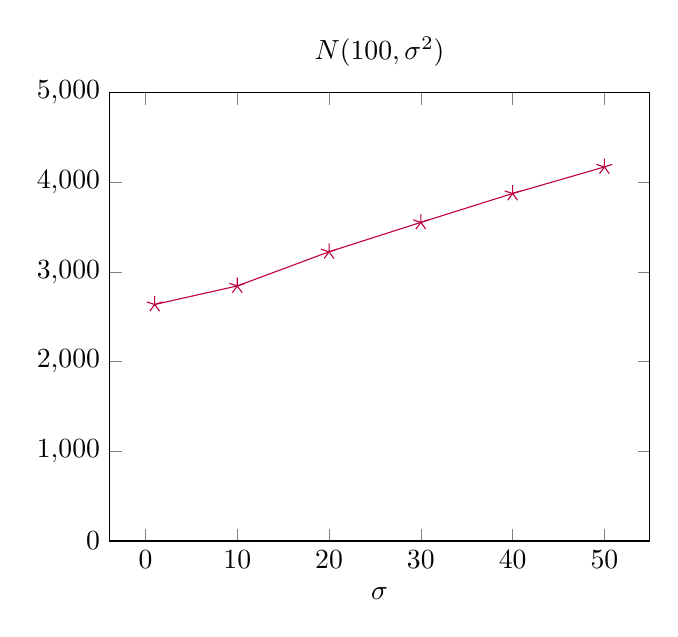
\begin{tikzpicture}
			\begin{axis}[
				title={$N(100,\sigma^2)$},
				x tick label style={draw=none},
				xlabel={$\sigma$},
				%ylabel={Total txns},
				ymin=0,
				ymax=5000,
				]
				\addplot[color=purple,mark=star,mark size=3pt] coordinates {(1,2638) (10,2845) (20,3226) (30,3554) (40,3876) (50,4172)};
			\end{axis}
		\end{tikzpicture}
	\end{minipage}
	\hspace{-80pt}
\end{document}